\documentclass[11pt,a4paper]{article}

% ========== Packages ==========
\usepackage[utf8]{inputenc}
\usepackage[T1]{fontenc}
\usepackage{amsmath,amsthm,amsfonts,amssymb}
\usepackage{mathtools}
\usepackage{bm}
% Algorithm environment using basic packages (no algorithm2e needed)
\usepackage{float}
\newfloat{algorithm}{tbp}{loa}
\floatname{algorithm}{Algorithm}
\usepackage{graphicx}
\usepackage{hyperref}
\usepackage{cleveref}
\usepackage{booktabs}
\usepackage{enumitem}
\usepackage{xcolor}
\usepackage{tikz}
\usepackage{subcaption}
\usepackage{natbib}
\usepackage{geometry}

\geometry{margin=1in}

% ========== Theorem Environments ==========
\newtheorem{theorem}{Theorem}[section]
\newtheorem{lemma}[theorem]{Lemma}
\newtheorem{proposition}[theorem]{Proposition}
\newtheorem{corollary}[theorem]{Corollary}
\newtheorem{definition}[theorem]{Definition}
\newtheorem{remark}[theorem]{Remark}

% ========== Custom Commands ==========
\newcommand{\R}{\mathbb{R}}
\newcommand{\C}{\mathbb{C}}
\newcommand{\N}{\mathbb{N}}
\newcommand{\E}{\mathbb{E}}
\newcommand{\U}{\mathcal{U}}
\newcommand{\B}{\mathcal{B}}
\newcommand{\HH}{\mathcal{H}}
\newcommand{\LL}{\mathcal{L}}
\newcommand{\tr}{\text{Tr}}
\newcommand{\diag}{\text{diag}}
\newcommand{\skewop}{\text{skew}}
\newcommand{\norm}[1]{\left\| #1 \right\|}
\newcommand{\abs}[1]{\left| #1 \right|}
\newcommand{\inner}[2]{\langle #1, #2 \rangle}
\DeclareMathOperator*{\argmin}{arg\,min}

% ========== Title and Authors ==========
\title{\textbf{Möbius Quantum Ring: A Unitary Manifold Approach to Stable and Expressive Recurrent Dynamics}}

\author{
  Fan Bai\\
  \textit{School of Equipment Engineering, Shenyang Ligong University}\\
  \texttt{snowwind001@gmail.com}
}

\date{January 2026}

\begin{document}

\maketitle

% ========== Abstract ==========
\begin{abstract}
Deep neural networks, particularly recurrent models, face a fundamental trade-off between expressive power and the stability of signal propagation. While techniques like gating mechanisms and orthogonal constraints have provided partial solutions, they often introduce computational overhead or limit the model's capacity for complex feature mixing. Recent work on Manifold-Constrained Hyper-Connections (mHC) has shown promise by projecting weights onto the Birkhoff polytope (doubly stochastic matrices), yet this relies on iterative Sinkhorn-Knopp normalization.

In this paper, we introduce the \textbf{Möbius Quantum Ring (MQR)}, a novel recurrent architecture that fundamentally reframes network dynamics as a dissipative quantum system on a unitary manifold. The MQR architecture is built on three core principles: (1) \textbf{Implicit Geometric Constraint}: We parameterize the connection weights using the Unistochastic Manifold, where the weight matrix $H$ is defined as the element-wise modulus squared of a unitary matrix $U$ ($H_{ij} = |U_{ij}|^2$), analytically guaranteeing doubly stochastic properties without iterative projection; (2) \textbf{Continuous Dynamics with External Drive}: The MQR is a ``headless'' and ``tailless'' ring network, where input signals are injected via low-rank Hamiltonian perturbation (LoRA-style) as an external driving force; (3) \textbf{Holomorphic Equilibrium Propagation}: Learning occurs through a BPTT-free algorithm that updates the unitary matrix's phase via Lie algebra operations, enabling efficient training on the unitary manifold.

We provide rigorous mathematical proofs for MQR's global asymptotic stability and derive its efficient learning algorithm. By leveraging the geometric properties of unitary groups, MQR achieves a powerful synthesis of stability, expressivity, and computational efficiency, offering a new paradigm for designing deep recurrent models.
\end{abstract}

\textbf{Keywords:} Unitary networks, Doubly stochastic matrices, Equilibrium propagation, Manifold optimization, Recurrent neural networks, Quantum-inspired computing

% ========== 1. Introduction ==========
\section{Introduction}
\label{sec:introduction}

The capacity of deep neural networks to model complex, long-range dependencies is intrinsically linked to their ability to propagate signals and gradients through many layers or time steps without explosion or vanishment. In feed-forward networks, Residual Networks (ResNets) \citep{he2016deep} addressed this by introducing identity skip-connections, ensuring a baseline signal path. In recurrent neural networks (RNNs), this challenge is even more pronounced, leading to the development of sophisticated gating mechanisms like LSTMs \citep{hochreiter1997long} and GRUs \citep{cho2014learning}.

While effective, these solutions can be viewed as ``engineered fixes'' rather than foundational principles. A more geometrically-motivated line of inquiry has focused on constraining the network's weight matrices. Orthogonal RNNs \citep{arjovsky2016unitary,wisdom2016full}, for instance, enforce $W^T W = I$, guaranteeing perfect isometry and preventing gradient explosion/vanishing. However, this strict constraint can limit the network's expressivity and requires computationally expensive parameterization schemes.

A recent breakthrough, Manifold-Constrained Hyper-Connections (mHC) \citep{wang2025sparse}, relaxed orthogonal constraints by projecting weights onto the \textbf{Birkhoff polytope}---the set of doubly stochastic matrices. A doubly stochastic matrix $H$ preserves the $L_1$ norm of the input and has a spectral norm of one, making it an ideal candidate for stable signal propagation while allowing for rich feature mixing beyond simple rotations. The primary drawback of mHC is its reliance on the Sinkhorn-Knopp algorithm \citep{sinkhorn1967concerning}, an iterative procedure required during each forward pass.

\textbf{Research Question:} Can we achieve the desirable properties of a doubly stochastic connection matrix without the computational burden of iterative projection?

We answer this affirmatively by introducing the \textbf{Möbius Quantum Ring (MQR)}. Our key insight is to parameterize the weight matrix through the \textbf{Unistochastic Manifold}---the set of matrices $H$ such that $H_{ij} = |U_{ij}|^2$ for some unitary matrix $U$. This parameterization analytically guarantees doubly stochastic properties without any iterative normalization.

\subsection{Contributions}

Our main contributions are:
\begin{enumerate}[leftmargin=*]
    \item \textbf{Architectural Innovation}: We propose MQR, a ``headless, tailless'' recurrent architecture where dynamics are governed by doubly stochastic weights derived from the unistochastic manifold. Input is injected as a Hamiltonian perturbation, and output is obtained via local projective sampling.
    
    \item \textbf{Efficient Parameterization}: We show that the Cayley transform provides a bijective, differentiable mapping from skew-Hermitian matrices to unitary matrices, enabling efficient gradient-based optimization on the unitary manifold without matrix exponentials.
    
    \item \textbf{Holomorphic Equilibrium Propagation}: We derive a BPTT-free training algorithm that updates parameters in the Lie algebra space $\mathfrak{u}(n)$, completely avoiding backpropagation through the relaxation dynamics.
    
    \item \textbf{Theoretical Guarantees}: We prove that MQR dynamics form a contraction mapping, guaranteeing unique fixed-point convergence, and that unistochastic matrices form a proper subset of the Birkhoff polytope with enhanced structure.
\end{enumerate}

% ========== 2. Related Work ==========
\section{Related Work}
\label{sec:related}

\subsection{Stabilizing Deep Networks}

The problem of training very deep networks has been approached from multiple angles. Batch Normalization \citep{ioffe2015batch} and Layer Normalization \citep{ba2016layer} stabilize activations by normalizing intermediate representations. ResNets \citep{he2016deep} and Highway Networks \citep{srivastava2015highway} use skip connections to ensure gradient flow. DenseNets \citep{huang2017densely} propagate features through concatenation. All these methods can be seen as engineering solutions to the fundamental problem of signal preservation.

\subsection{Orthogonal and Unitary Networks}

A more principled approach enforces geometric constraints on weight matrices. Orthogonal RNNs \citep{arjovsky2016unitary} maintain $W^TW = I$, guaranteeing isometry. Unitary Evolution RNNs \citep{wisdom2016full} extend this to complex-valued unitary matrices. The Cayley transform \citep{helfrich2018orthogonal} and Householder parameterizations \citep{mhammedi2017efficient} provide efficient methods to maintain orthogonality during training. Our work builds upon this foundation but relaxes strict orthogonality to the more expressive unistochastic constraint.

\subsection{Doubly Stochastic Matrices and Birkhoff Polytope}

Doubly stochastic matrices have been used in attention mechanisms \citep{sander2022sinkformers} and optimal transport \citep{cuturi2013sinkhorn}. The mHC framework \citep{wang2025sparse} constrains hyper-connection weights to the Birkhoff polytope via Sinkhorn iterations. Our unistochastic approach can be seen as selecting a geometrically-privileged subset of the Birkhoff polytope that admits closed-form parameterization.

\subsection{Equilibrium Models}

Implicit deep learning models define output as the fixed point of a dynamical system \citep{bai2019deep,amos2017optnet}. Equilibrium Propagation \citep{scellier2017equilibrium} provides a biologically-plausible learning rule for such systems. Our Holomorphic Equilibrium Propagation extends these ideas to complex-valued dynamics with manifold constraints.

% ========== 3. Mathematical Preliminaries ==========
\section{Mathematical Preliminaries}
\label{sec:preliminaries}

\subsection{Unitary Group and Lie Algebra}

\begin{definition}[Unitary Group]
The unitary group $U(n)$ consists of all $n \times n$ complex matrices $U$ satisfying $U^\dagger U = U U^\dagger = I$, where $U^\dagger$ denotes the conjugate transpose.
\end{definition}

\begin{definition}[Lie Algebra $\mathfrak{u}(n)$]
The Lie algebra of $U(n)$ is the set of skew-Hermitian matrices:
\begin{equation}
\mathfrak{u}(n) = \{A \in \C^{n \times n} : A^\dagger = -A\}
\end{equation}
\end{definition}

The exponential map $\exp: \mathfrak{u}(n) \to U(n)$ maps Lie algebra elements to the group:
\begin{equation}
\exp(A) = \sum_{k=0}^\infty \frac{A^k}{k!}
\end{equation}

For skew-Hermitian $A$, $\exp(A)$ is always unitary.

\subsection{Cayley Transform}

While the matrix exponential is mathematically elegant, it is computationally expensive. The \textbf{Cayley transform} provides an alternative:

\begin{proposition}[Cayley Transform]
\label{prop:cayley}
For any skew-Hermitian matrix $A \in \mathfrak{u}(n)$, the matrix
\begin{equation}
U = (I - A)(I + A)^{-1}
\end{equation}
is unitary. The inverse relationship is $A = (I - U)(I + U)^{-1}$.
\end{proposition}

\begin{proof}
We verify $U^\dagger U = I$:
\begin{align}
U^\dagger U &= [(I - A)(I + A)^{-1}]^\dagger [(I - A)(I + A)^{-1}] \notag \\
&= (I + A^\dagger)^{-1}(I - A^\dagger)(I - A)(I + A)^{-1} \notag \\
&= (I - A)^{-1}(I + A)(I - A)(I + A)^{-1} \quad (\text{since } A^\dagger = -A) \notag \\
&= I
\end{align}
Similarly, $U U^\dagger = I$.
\end{proof}

\subsection{Birkhoff Polytope and Doubly Stochastic Matrices}

\begin{definition}[Birkhoff Polytope]
The Birkhoff polytope $\B_n$ is the set of $n \times n$ doubly stochastic matrices:
\begin{equation}
\B_n = \{H \in \R^{n \times n}_{\geq 0} : H\mathbf{1} = \mathbf{1}, H^T\mathbf{1} = \mathbf{1}\}
\end{equation}
where $\mathbf{1}$ is the all-ones vector.
\end{definition}

Doubly stochastic matrices have several important properties:
\begin{itemize}
    \item \textbf{Spectral Norm}: $\|H\|_2 \leq 1$ with equality iff $H$ is a permutation matrix.
    \item \textbf{$L_1$ Preservation}: For any $x \geq 0$, $\|Hx\|_1 = \|x\|_1$.
    \item \textbf{Convexity}: $\B_n$ is a convex polytope with permutation matrices as vertices (Birkhoff-von Neumann theorem).
\end{itemize}

\subsection{Unistochastic Manifold}

\begin{definition}[Unistochastic Matrix]
A matrix $H \in \R^{n \times n}$ is unistochastic if there exists a unitary matrix $U \in U(n)$ such that:
\begin{equation}
H_{ij} = |U_{ij}|^2
\end{equation}
The set of all unistochastic matrices is denoted $\U_n$.
\end{definition}

The following theorem establishes the key property:

\begin{theorem}
\label{thm:unistochastic}
Any unistochastic matrix is doubly stochastic: $\U_n \subset \B_n$.
\end{theorem}

\begin{proof}
Let $H_{ij} = |U_{ij}|^2$ for some unitary $U$.

\textbf{Non-negativity:} $H_{ij} = |U_{ij}|^2 \geq 0$. \checkmark

\textbf{Row Sums:} From $UU^\dagger = I$, we have $(UU^\dagger)_{ii} = 1$:
\begin{equation}
\sum_{j=1}^n U_{ij} \overline{U_{ij}} = \sum_{j=1}^n |U_{ij}|^2 = \sum_{j=1}^n H_{ij} = 1
\end{equation}

\textbf{Column Sums:} From $U^\dagger U = I$, we have $(U^\dagger U)_{jj} = 1$:
\begin{equation}
\sum_{i=1}^n \overline{U_{ij}} U_{ij} = \sum_{i=1}^n |U_{ij}|^2 = \sum_{i=1}^n H_{ij} = 1
\end{equation}
\end{proof}

\begin{remark}
Not every doubly stochastic matrix is unistochastic. For example, the $3 \times 3$ doubly stochastic matrix with all entries equal to $1/3$ is not unistochastic \citep{bengtsson2005birkhoff}. Thus $\U_n \subsetneq \B_n$ for $n \geq 3$.
\end{remark}

% ========== 4. The Möbius Quantum Ring Architecture ==========
\section{The Möbius Quantum Ring Architecture}
\label{sec:architecture}

\subsection{Conceptual Overview}

The Möbius Quantum Ring (MQR) departs from traditional feed-forward or sequential recurrent architectures. Instead, we construct a ``headless, tailless'' dynamical system:

\begin{itemize}
    \item \textbf{No explicit input layer}: Inputs are injected as perturbations to the system's dynamics.
    \item \textbf{No explicit output layer}: Outputs are obtained by sampling local regions of the steady-state.
    \item \textbf{Fixed-point computation}: The network's ``forward pass'' is an iterative relaxation to equilibrium.
\end{itemize}

This design is inspired by physical systems where steady-state observations emerge from continuous dynamics rather than discrete layer-wise computation.

\subsection{State Dynamics}

Let $h \in \R^N$ denote the ring's hidden state vector, where $N$ is the number of nodes. The state evolution follows:

\begin{equation}
\label{eq:dynamics}
h_{t+1} = (1 - \alpha) H^T h_t + \alpha J(x)
\end{equation}

where:
\begin{itemize}
    \item $H \in \U_N$ is the unistochastic connection matrix, $H = |U|^2$
    \item $\alpha \in (0, 1]$ is the injection strength (damping coefficient)
    \item $J(x) \in \R^N$ is the injection signal derived from input $x$
\end{itemize}

The dynamics can be written as an affine map $T(h) = (1-\alpha)H^Th + \alpha J(x)$.

\subsection{Hamiltonian Injection (LoRA-Style)}

Instead of directly setting an initial state, we inject the input as an external ``Hamiltonian perturbation'' using a low-rank decomposition:

\begin{equation}
\label{eq:injection}
J(x) = W_{up} W_{down} x
\end{equation}

where $W_{down} \in \R^{r \times d}$ and $W_{up} \in \R^{N \times r}$ with rank $r \ll \min(N, d)$. This is reminiscent of LoRA \citep{hu2021lora} and can be interpreted as adding an external potential that drives the system.

\subsection{Local Projective Readout}

Output is obtained by ``measuring'' a local subset of the steady-state:

\begin{equation}
\label{eq:readout}
y = W_{readout} \cdot h^*_S
\end{equation}

where $h^*$ is the fixed point and $S \subset \{1, \ldots, N\}$ is the set of sampled node indices. This mimics quantum measurement, where only partial information is extracted from the full state.

\subsection{Unitary Parameterization via Cayley Transform}

The unitary matrix $U$ is parameterized through a skew-Hermitian matrix $A$:

\begin{equation}
A = \frac{1}{2}\left[(R - R^T) + i(S + S^T)\right]
\end{equation}

where $R, S \in \R^{N \times N}$ are learnable parameters. This ensures $A^\dagger = -A$ by construction. The unitary matrix is then:

\begin{equation}
U = (I - A)(I + A)^{-1}
\end{equation}

And the unistochastic weight matrix:

\begin{equation}
H = |U|^2 \quad \text{(element-wise)}
\end{equation}

\begin{algorithm}[t]
\caption{MQR Forward Pass}
\label{alg:forward}
\begin{tabular}{@{}l@{}}
\textbf{Input:} $x \in \R^d$, parameters $A, W_{down}, W_{up}, W_{readout}$ \\
\textbf{Input:} Hyperparameters: $\alpha$, relaxation steps $K$, sample indices $S$ \\[0.5em]
1: Construct skew-Hermitian $A$ from parameters \\
2: $U \gets (I - A)(I + A)^{-1}$ \hfill \textit{// Cayley transform} \\
3: $H \gets |U|^2$ \hfill \textit{// Unistochastic matrix} \\
4: $J \gets W_{up} W_{down} x$ \hfill \textit{// Hamiltonian injection} \\
5: $h \gets \mathbf{0}$ \hfill \textit{// Initialize state} \\
6: \textbf{for} $k = 1$ \textbf{to} $K$ \textbf{do} \\
7: \quad $h \gets (1-\alpha)H^T h + \alpha J$ \hfill \textit{// Relaxation step} \\
8: \textbf{end for} \\
9: $y \gets W_{readout} \cdot h_S$ \hfill \textit{// Local projective readout} \\
10: \textbf{return} $y$ \\
\end{tabular}
\end{algorithm}

% ========== 5. Theoretical Analysis ==========
\section{Theoretical Analysis}
\label{sec:theory}

\subsection{Fixed-Point Existence and Uniqueness}

\begin{theorem}[Contraction Mapping]
\label{thm:contraction}
For $\alpha \in (0, 1]$, the map $T(h) = (1-\alpha)H^T h + \alpha J$ is a contraction on $\R^N$ with respect to the $\ell_\infty$ norm.
\end{theorem}

\begin{proof}
For any $h_1, h_2 \in \R^N$:
\begin{align}
\|T(h_1) - T(h_2)\|_\infty &= \|(1-\alpha)H^T(h_1 - h_2)\|_\infty \notag \\
&\leq (1-\alpha)\|H^T\|_\infty \|h_1 - h_2\|_\infty
\end{align}

Since $H$ is doubly stochastic, $\|H^T\|_\infty = \max_i \sum_j H_{ji} = 1$. Therefore:
\begin{equation}
\|T(h_1) - T(h_2)\|_\infty \leq (1-\alpha)\|h_1 - h_2\|_\infty
\end{equation}

For $\alpha > 0$, we have $1 - \alpha < 1$, so $T$ is a contraction.
\end{proof}

\begin{corollary}[Unique Fixed Point]
By the Banach Fixed-Point Theorem, there exists a unique fixed point $h^*$ satisfying:
\begin{equation}
h^* = (1-\alpha)H^T h^* + \alpha J \quad \Rightarrow \quad h^* = \alpha(I - (1-\alpha)H^T)^{-1}J
\end{equation}
\end{corollary}

\subsection{Spectral Analysis}

\begin{theorem}[Spectral Radius Bound]
\label{thm:spectral}
For unistochastic $H$, the eigenvalues $\lambda$ of $(1-\alpha)H^T$ satisfy $|\lambda| \leq 1 - \alpha$.
\end{theorem}

\begin{proof}
Since $H$ is doubly stochastic:
\begin{enumerate}
    \item $H$ has spectral radius $\rho(H) \leq \|H\|_\infty = 1$.
    \item The eigenvalue $\lambda = 1$ corresponds to the stationary distribution.
    \item For $(1-\alpha)H^T$, eigenvalues are scaled: $\tilde{\lambda} = (1-\alpha)\lambda$.
    \item Thus $|\tilde{\lambda}| \leq (1-\alpha) < 1$ for $\alpha > 0$.
\end{enumerate}
\end{proof}

This spectral bound ensures:
\begin{itemize}
    \item \textbf{No gradient explosion}: Eigenvalues strictly inside unit circle.
    \item \textbf{Exponential convergence}: $\|h_t - h^*\| = O((1-\alpha)^t)$.
\end{itemize}

\subsection{Energy Conservation}

\begin{proposition}[$L_1$ Norm Bounds]
\label{prop:l1bounds}
For any $h \geq 0$ (element-wise), we have $\|H^Th\|_1 = \|h\|_1$.
\end{proposition}

\begin{proof}
\begin{equation}
\|H^Th\|_1 = \sum_i \sum_j H_{ji}h_j = \sum_j h_j \sum_i H_{ji} = \sum_j h_j = \|h\|_1
\end{equation}
where we used the column-sum property of doubly stochastic matrices.
\end{proof}

This property ensures that the ``energy'' (measured as $L_1$ norm) of non-negative signals is perfectly conserved during propagation.

% ========== 6. Holomorphic Equilibrium Propagation ==========
\section{Holomorphic Equilibrium Propagation}
\label{sec:learning}

\subsection{The Learning Challenge}

Standard backpropagation through the relaxation dynamics \eqref{eq:dynamics} requires unrolling $K$ iterations and storing intermediate states---computationally expensive and memory-intensive. We propose \textbf{Holomorphic Equilibrium Propagation}, a BPTT-free algorithm that exploits the fixed-point structure.

\subsection{Adjoint State Computation}

At the fixed point $h^*$, implicit differentiation gives:

\begin{equation}
\frac{\partial h^*}{\partial \theta} = (I - (1-\alpha)H^T)^{-1} \frac{\partial [(1-\alpha)H^T h^* + \alpha J]}{\partial \theta}
\end{equation}

Rather than computing this inverse explicitly, we solve for the \textbf{adjoint state} $h^\dagger$ via a dual fixed-point iteration:

\begin{equation}
\label{eq:adjoint}
h^\dagger = (1-\alpha)H h^\dagger + \alpha \nabla_{h^*}\LL
\end{equation}

where $\nabla_{h^*}\LL$ is the gradient of the loss with respect to the fixed point (computed at the readout layer).

\begin{proposition}
The adjoint iteration \eqref{eq:adjoint} converges to the solution of:
\begin{equation}
h^\dagger = (I - (1-\alpha)H)^{-1} \alpha \nabla_{h^*}\LL
\end{equation}
\end{proposition}

\subsection{Gradient with Respect to $H$}

Once $h^*$ and $h^\dagger$ are computed, the gradient with respect to $H$ is approximated as:

\begin{equation}
\frac{\partial \LL}{\partial H} \approx (h^\dagger)^T h^* = h^\dagger \otimes h^*
\end{equation}

where $\otimes$ denotes outer product.

\subsection{Lie Algebra Update}

The key innovation is mapping the gradient from $H$ back to the Lie algebra $\mathfrak{u}(n)$. Since $H_{ij} = |U_{ij}|^2 = U_{ij}\bar{U}_{ij}$, we have:

\begin{equation}
\frac{\partial \LL}{\partial U} = \frac{\partial \LL}{\partial H} \odot \bar{U}
\end{equation}

To update the skew-Hermitian parameter $A$, we project this onto the tangent space at $U$:

\begin{equation}
\label{eq:deltaA}
\Delta A \propto \text{skew}\left(U^\dagger \cdot \left(\frac{\partial \LL}{\partial H} \odot U \odot \bar{U}\right)\right)
\end{equation}

where $\text{skew}(M) = \frac{1}{2}(M - M^\dagger)$ extracts the skew-Hermitian part.

\begin{remark}[Comparison with Exponential Map]
An alternative update is $U_{new} = \exp(-i\eta\Omega)U_{old}$, which directly operates on the Lie group via the exponential map. While geometrically elegant, this requires computing a matrix exponential. Our $\Delta A$ update achieves similar effects with only matrix multiplication, as the Cayley transform automatically ``projects back'' to the unitary group.
\end{remark}

\begin{algorithm}[t]
\caption{Holomorphic Equilibrium Propagation (One Step)}
\label{alg:heqprop}
\begin{tabular}{@{}l@{}}
\textbf{Input:} Batch $(x, y_{target})$, learning rate $\eta$ \\
\textbf{Input:} Current parameters $A, W_{down}, W_{up}, W_{readout}$ \\[0.5em]
\textit{// Phase 1: Forward to Fixed Point} \\
1: Compute $U, H, J$ as in Algorithm~\ref{alg:forward} \\
2: Run relaxation to obtain $h^*$ \\
3: Compute output $\hat{y} = W_{readout} \cdot h^*_S$ \\
4: Compute loss $\LL = \text{CrossEntropy}(\hat{y}, y_{target})$ \\[0.3em]
\textit{// Phase 2: Adjoint Fixed Point} \\
5: Compute $\nabla_{\hat{y}}\LL$ (softmax gradient) \\
6: $\nabla_{h^*}\LL \gets$ scatter $W_{readout}^T \nabla_{\hat{y}}\LL$ to full dimension \\
7: Initialize $h^\dagger \gets \mathbf{0}$ \\
8: \textbf{for} $k = 1$ \textbf{to} $K_{adj}$ \textbf{do} \\
9: \quad $h^\dagger \gets (1-\alpha)H h^\dagger + \alpha \nabla_{h^*}\LL$ \\
10: \textbf{end for} \\[0.3em]
\textit{// Phase 3: Parameter Updates} \\
11: $\nabla_H\LL \gets (h^\dagger)^T h^*$ \\
12: $M \gets U^\dagger \cdot (\nabla_H\LL \odot H)$ \\
13: $\Delta A \gets \text{skew}(M)$ \\
14: $A \gets A - \eta \cdot \Delta A$ \hfill \textit{// Lie algebra update} \\
15: Update $W_{readout}, W_{up}, W_{down}$ with standard gradients \\
16: \textbf{return} Updated parameters \\
\end{tabular}
\end{algorithm}

\subsection{Injection and Readout Updates}

The LoRA-style injection parameters are updated via chain rule:

\begin{align}
\nabla_{W_{up}}\LL &= (h^\dagger)^T \cdot z \quad \text{where } z = W_{down}x \\
\nabla_{W_{down}}\LL &= (W_{up}^T h^\dagger)^T \cdot x
\end{align}

The readout parameters are updated as:
\begin{equation}
\nabla_{W_{readout}}\LL = (\nabla_{\hat{y}}\LL)^T \cdot h^*_S
\end{equation}

% ========== 7. Online Dual-Loop Extensions ==========
\section{Online Dual-Loop Dynamics and Dual-Unitary Decomposition}
\label{sec:o2ep}

This section formalizes an \textbf{online alternating inference--training} regime and an architectural refinement that separates a frozen \emph{world model} from a learnable \emph{policy}. The goal is to better reflect the ``cognitive-reflection'' interpretation discussed in the source specification: every time step performs one forward relaxation (fast inference), and, only when external feedback (GT) exists, performs a reverse-ring update (learning).

\subsection{Online Alternating Inference--Training (O2EP)}

At each discrete time $t$, we receive an input $x_t$ and optionally a supervisory signal $y_t$ (or more generally, a target distribution). Define the forward relaxation map
\begin{equation}
\Phi_t(h) \triangleq (1-\alpha)\,hH_t^T + \alpha J(x_t),
\end{equation}
where $H_t$ is the current unistochastic coupling (Sec.~\ref{sec:architecture}). Under the same assumptions as Theorem~\ref{thm:contraction}, $\Phi_t$ is a contraction (in $\|\cdot\|_\infty$), hence the fixed point $h_t^*$ exists and is unique. The online forward pass is simply $h_t^*=\text{FixPoint}(\Phi_t)$.

If a target is present, we compute the loss $\LL_t$ and solve an adjoint fixed point (Sec.~\ref{sec:learning}) to obtain $h_t^\dagger$, then update parameters with one ``reverse-ring'' step. If no target is present, we skip learning and only output $\hat{y}_t$.

\subsection{Dual Unitary Factorization: World Model \& Policy}

We decompose the unitary that induces the coupling as
\begin{equation}
U_{\text{total}} = U_{\text{policy}}\,U_{\text{base}}, \qquad U_{\text{base}}\in U(N)\ \text{frozen.}
\end{equation}
The learnable part $U_{\text{policy}}$ is parameterized by a skew-Hermitian $A_{\text{policy}}\in\mathfrak{u}(N)$ via the Cayley transform (Sec.~\ref{sec:preliminaries}), while $U_{\text{base}}$ remains fixed over the task/episode.

\begin{proposition}[Preservation of Unitarity and Unistochasticity]
\label{prop:dual_unitary}
If $U_{\text{policy}}\in U(N)$ and $U_{\text{base}}\in U(N)$, then $U_{\text{total}}\in U(N)$. Consequently, $H=|U_{\text{total}}|^2$ is doubly stochastic.
\end{proposition}

\begin{proof}
Unitarity follows from closure of $U(N)$ under multiplication:
$(U_{\text{total}})^\dagger U_{\text{total}} = U_{\text{base}}^\dagger(U_{\text{policy}}^\dagger U_{\text{policy}})U_{\text{base}} = I$.
The doubly stochastic property of $H=|U|^2$ for unitary $U$ is given in Sec.~\ref{sec:preliminaries} (unistochastic manifold discussion).
\end{proof}

This separation implements a \emph{stability--plasticity} design: the forward ``physics'' is anchored by $U_{\text{base}}$, while adaptation occurs through $U_{\text{policy}}$.

\subsection{Learnable Goal Equilibrium State}

Beyond a readout loss on $\hat{y}$, we may impose a state-level objective. Let $P\in\mathbb{R}^{C\times N}$ be a set of \textbf{learnable goal equilibria} (e.g., one prototype $p_y$ per class). A simple goal-matching term is:
\begin{equation}
\LL_{\text{state}}(h_t^*, y_t) = \frac{1}{2}\|h_t^* - p_{y_t}\|_2^2,
\end{equation}
and we optimize $\LL_t = \LL_{\text{cls}} + \lambda\,\LL_{\text{state}}$.
This explicitly models ``education'': the reverse ring nudges the system toward an internally represented desired equilibrium while also learning the goal itself (via updates to $P$).

\subsection{Prototype-Distance Readout (Goal-Aligned Logits)}

In practice, a potential mismatch arises if the classifier logits are produced by a separate linear readout while the goal is defined in state space. To directly tie decision-making to goal equilibria, we introduce an optional \textbf{prototype-distance readout} on the sampled subspace $S$:
\begin{equation}
\label{eq:proto_logits}
\hat{y}_{t,c} \;=\; -\frac{1}{2\tau}\,\|h_{t,S}^* - p_{c,S}\|_2^2,
\end{equation}
where $\tau>0$ is a temperature. This preserves the ``local measurement'' principle (Sec.~\ref{sec:architecture}) while making classification gradients act directly on the goal states.

\begin{proposition}[Gradient Source for Prototype Readout]
\label{prop:proto_grad}
Let $g_t=\nabla_{\hat{y}_t}\LL_t\in\mathbb{R}^{C}$ be the softmax-gradient at time $t$. For \eqref{eq:proto_logits}, the gradient on the sampled state is
\begin{equation}
\nabla_{h_{t,S}^*}\LL_t \;=\; -\frac{1}{\tau}\left(h_{t,S}^*\,\mathbf{1}^T g_t - P_S^T g_t\right),
\end{equation}
and the gradient on prototypes is
\begin{equation}
\nabla_{P_S}\LL_t \;=\; \frac{1}{\tau}\left(g_t\, (h_{t,S}^*)^T - \operatorname{diag}(g_t)\,P_S\right),
\end{equation}
where $P_S\in\mathbb{R}^{C\times |S|}$ is the prototype matrix restricted to $S$ and $\mathbf{1}$ is an all-ones vector.
\end{proposition}

\begin{proof}
For each class $c$, $\hat{y}_{t,c}=-(2\tau)^{-1}\|h_{t,S}^*-p_{c,S}\|_2^2$. Thus
$\partial \hat{y}_{t,c}/\partial h_{t,S}^* = -\tau^{-1}(h_{t,S}^*-p_{c,S})$ and
$\partial \hat{y}_{t,c}/\partial p_{c,S} = \tau^{-1}(h_{t,S}^*-p_{c,S})$.
Multiplying by $g_{t,c}=\partial \LL_t/\partial \hat{y}_{t,c}$ and summing over $c$ yields the stated expressions.
\end{proof}

\subsection{Algorithm: Online Orthogonal Equilibrium Propagation (O2EP)}

\begin{algorithm}[t]
\caption{Online Dual-Loop MQR (O2EP) at Time $t$}
\label{alg:o2ep}
\begin{tabular}{@{}l@{}}
\textbf{Input:} $x_t$, optional $y_t$, step size $\eta$ \\
\textbf{State:} previous $h_{t-1}^*$ (optional warm start) \\[0.3em]
\textit{// Forward ring (always)} \\
1: Form $U_{\text{total}}=U_{\text{policy}}U_{\text{base}}$, $H=|U_{\text{total}}|^2$, and $J(x_t)$ \\
2: Relax $h\leftarrow (1-\alpha)hH^T+\alpha J(x_t)$ for $K$ steps to get $h_t^*$ \\
3: Produce logits $\hat{y}_t$ (linear readout or prototype readout on $S$) \\[0.3em]
\textit{// Reverse ring (only if GT exists)} \\
4: \textbf{if} $y_t$ exists \textbf{then} \\
5:\quad Compute loss $\LL_t$ and $\nabla_{h_t^*}\LL_t$ (Prop.~\ref{prop:proto_grad} if using prototypes) \\
6:\quad Solve $h_t^\dagger=(1-\alpha)Hh_t^\dagger+\alpha\nabla_{h_t^*}\LL_t$ for $K_{adj}$ steps \\
7:\quad $\nabla_H\LL_t \gets (h_t^\dagger)^T h_t^*$ \\
8:\quad Update $A_{\text{policy}}$ using the Lie algebra step \eqref{eq:deltaA} (with $U_{\text{total}}$ pullback) \\
9:\quad Update injection/readout (and prototypes if enabled) \\
10: \textbf{end if} \\
\textbf{return} $\hat{y}_t$, $h_t^*$ \\
\end{tabular}
\end{algorithm}

% ========== 8. Expressivity Extensions ==========
\section{Expressivity Extensions for Vision Tasks}
\label{sec:extensions}

The strict MQR formulation (Sec.~\ref{sec:architecture}--\ref{sec:learning}) emphasizes stability and geometric constraints. For challenging vision benchmarks (e.g., CIFAR-100), the base ``flatten $\rightarrow$ low-rank injection $\rightarrow$ ring $\rightarrow$ local readout'' pipeline can be under-expressive. This section records three \emph{optional} extensions implemented in our codebase that improve representational power while preserving the core ``ring + fixed point + EQProp'' principle.

\subsection{Nonlinear Fixed-Point Dynamics with 1-Lipschitz Activations}
\label{sec:ext_nonlinear}

We may insert an element-wise activation $\sigma$ inside the relaxation:
\begin{equation}
h_{k+1} \;=\; \sigma\!\left((1-\alpha)\,h_k H^T + \alpha\,J(x)\right).
\end{equation}
If $\sigma$ is 1-Lipschitz under $\|\cdot\|_\infty$ (e.g., ReLU, $\tanh$), the Banach fixed-point guarantee remains intact.

\begin{theorem}[Contraction with 1-Lipschitz Activation]
Let $H$ be doubly stochastic and $0<\alpha\le 1$. If $\sigma$ satisfies $\|\sigma(u)-\sigma(v)\|_\infty\le \|u-v\|_\infty$, then the map
$\Phi(h)=\sigma((1-\alpha)hH^T+\alpha J)$ is a contraction with constant $(1-\alpha)$ in $\|\cdot\|_\infty$.
\end{theorem}

\begin{proof}
For any $h_1,h_2$, using 1-Lipschitzness and $\|H^T\|_\infty=1$,
\begin{align}
\|\Phi(h_1)-\Phi(h_2)\|_\infty
&\le \|(1-\alpha)(h_1-h_2)H^T\|_\infty \\
&\le (1-\alpha)\|h_1-h_2\|_\infty.
\end{align}
\end{proof}

The corresponding adjoint iteration gains a local Jacobian factor $\sigma'(h^*)$:
\begin{equation}
h^\dagger \;=\; (1-\alpha)\,(h^\dagger \odot \sigma'(h^*))\,H \;+\; \alpha\,\nabla_{h^*}\LL,
\end{equation}
which is the form used in our implementation.

\subsection{Patch Embedding Front-End (Local Receptive Field)}
\label{sec:ext_patch}

To mitigate the ``raw pixel flattening'' bottleneck, we add an optional patch embedding encoder before the ring. For patch size $p$, a stride-$p$ convolution produces patch tokens:
\begin{equation}
E(x) \in \mathbb{R}^{P\times d_p},\quad P=(H/p)(W/p),
\end{equation}
followed by per-token normalization. The ring input vector is then obtained by pooling (mean) or flattening:
\begin{equation}
\tilde{x} =
\begin{cases}
\frac{1}{P}\sum_{j=1}^P E(x)_j, & \text{mean pool}\\
\operatorname{vec}(E(x)), & \text{flatten.}
\end{cases}
\end{equation}
We keep the ring dynamics unchanged and simply replace $x$ with $\tilde{x}$ in $J(\cdot)$.

\subsection{Self-Retention Mixing of Unistochastic Coupling}
\label{sec:ext_beta}

Pure doubly-stochastic propagation can exhibit an ``over-mixing'' tendency, pushing states toward uniformity when iterated many times. We therefore introduce an optional self-retention interpolation:
\begin{equation}
H_{\text{eff}} \;=\; (1-\beta)I + \beta H,\qquad \beta\in[0,1].
\end{equation}

\begin{proposition}[Doubly Stochasticity Preserved]
If $H$ is doubly stochastic, then $H_{\text{eff}}$ is doubly stochastic for any $\beta\in[0,1]$.
\end{proposition}

\begin{proof}
Both $I$ and $H$ have row/column sums equal to 1. A convex combination preserves these sums, hence $H_{\text{eff}}$ is doubly stochastic.
\end{proof}

The contraction theorem (Thm.~\ref{thm:contraction} and Sec.~\ref{sec:ext_nonlinear}) remains unchanged because $\|H_{\text{eff}}^T\|_\infty=1$. In learning, the chain rule yields $\nabla_H\LL = \beta\,\nabla_{H_{\text{eff}}}\LL$, and $\beta$ itself can be treated as a hyperparameter or learned.

\subsection{Complex Unitary Dynamics and Measurement Nonlinearity}
\label{sec:ext_unitary}

The strict MQR inference uses $H=|U|^2$, which discards phase in the forward relaxation. To let phase participate in inference, we provide an alternative \emph{complex} relaxation:
\begin{equation}
h_{k+1} \;=\; (1-\alpha)\,h_k U^\dagger + \alpha\,J(x), \qquad h_k\in\mathbb{C}^N,
\end{equation}
where $U\in U(N)$ is unitary and we use row-vector convention (right multiplication). Since $\|hU^\dagger\|_2=\|h\|_2$, this map is a contraction in $\|\cdot\|_2$ with constant $(1-\alpha)$.

We define a \emph{measurement} $m=\mathcal{M}(h^*)\in\mathbb{R}^N$ for readout and state-level losses. In our implementation, $\mathcal{M}(h)=|h|$ (element-wise magnitude). Then logits are computed from $m_S$ (linear) or distances to prototypes in $m$-space (Sec.~\ref{sec:o2ep}). This reintroduces a controlled nonlinearity even though the complex relaxation is linear.

The adjoint for the complex relaxation uses the adjoint operator of $U^\dagger$, i.e., $U$:
\begin{equation}
h^\dagger \;=\; (1-\alpha)\,h^\dagger U + \alpha\,\nabla_{h^*}\LL,
\end{equation}
where $\nabla_{h^*}\LL$ is obtained by pulling back the measurement gradient via $\mathcal{M}$. A convenient outer-product form for the unitary gradient is
\begin{equation}
\nabla_U \LL \;\propto\; (h^\dagger)^\dagger h^*,
\end{equation}
followed by tangent projection on $U(N)$:
\begin{equation}
\Delta A \;\propto\; \skewop\!\left(U^\dagger\,\nabla_U\LL\right),\qquad A\in\mathfrak{u}(N),
\end{equation}
with the same $U_{\text{total}}=U_{\text{policy}}U_{\text{base}}$ pullback logic as Sec.~\ref{sec:o2ep}.

% ========== 7. Computational Complexity ==========
\section{Computational Complexity}
\label{sec:complexity}

\subsection{Forward Pass}

\begin{table}[h]
\centering
\begin{tabular}{lcc}
\toprule
\textbf{Operation} & \textbf{Complexity} & \textbf{Notes} \\
\midrule
Cayley Transform & $O(N^3)$ & Matrix solve \\
Compute $H = |U|^2$ & $O(N^2)$ & Element-wise \\
Injection $J = W_{up}W_{down}x$ & $O(Nr + rd)$ & Low-rank \\
Relaxation ($K$ steps) & $O(KN^2)$ & Matrix-vector \\
Readout & $O(|S| \cdot C)$ & Linear layer \\
\bottomrule
\end{tabular}
\caption{Forward pass complexity for input dimension $d$, hidden $N$, classes $C$, rank $r$, sample size $|S|$, and relaxation steps $K$.}
\label{tab:complexity_forward}
\end{table}

\subsection{Comparison with mHC}

\begin{table}[h]
\centering
\begin{tabular}{lcc}
\toprule
\textbf{Method} & \textbf{Normalization} & \textbf{Complexity per Forward} \\
\midrule
mHC (Sinkhorn) & $O(T_{sink} N^2)$ & Iterative, $T_{sink} \sim 10$-$100$ \\
MQR (Cayley) & $O(N^3)$ & Single matrix solve \\
\bottomrule
\end{tabular}
\caption{Comparison of normalization costs.}
\label{tab:comparison}
\end{table}

For large $N$, the single $O(N^3)$ Cayley solve is often faster than repeated $O(N^2)$ Sinkhorn iterations, and admits more efficient GPU parallelization.

% ========== 8. Experiments ==========
\section{Experiments}
\label{sec:experiments}

\subsection{Experimental Setup}
\label{sec:exp_setup}

We evaluate the proposed Möbius Quantum Ring (MQR) on CIFAR-100 (50k train / 10k test, 100 classes) using Top-1 accuracy.
Our goal is not to claim a new state-of-the-art, but to validate the \emph{functional viability} of MQR as a stable, replaceable module under the ``C-strategy'': a strong visual backbone provides representations, and MQR acts as a head that can be expanded progressively.

\paragraph{C-strategy model (ViT backbone + MQR head).}
Unless otherwise stated, we use a small ViT backbone with patch size $4$ and CLS pooling, and attach an MQR head.
The MQR uses hidden dimension $N=192$, relaxation steps $K=12$, and $\alpha=0.3$.
Input injection is implemented via a LoRA-style low-rank perturbation (rank $r=128$) with ReLU injection activation and a tanh state activation.
We use $H$-mix (Sec.~\ref{sec:ext_hmix}) with $\beta=0.6$ and learn $\beta$ jointly.

\paragraph{Optimization and schedule.}
We update the MQR head using Holomorphic Equilibrium Propagation (Sec.~\ref{sec:eqprop}) and update the ViT encoder using AdamW, driven by the gradient $\nabla_x\LL$ returned from the MQR EQProp step.
We use a cosine learning-rate schedule with linear warmup (1 epoch) and a minimum learning-rate ratio of 0.01.
For the main ViT+MQR setting, we use learning rate $3\times 10^{-3}$, batch size 64, and train up to 500 epochs.
We apply standard modern augmentation/regularization: label smoothing 0.1, Mixup (prob 0.5, $\alpha=0.2$), and CutMix (prob 0.5, $\alpha=1.0$).

\subsection{Main Result: ViT Backbone + MQR Head (C-strategy)}
\label{sec:exp_main}

\begin{figure}[t]
\centering
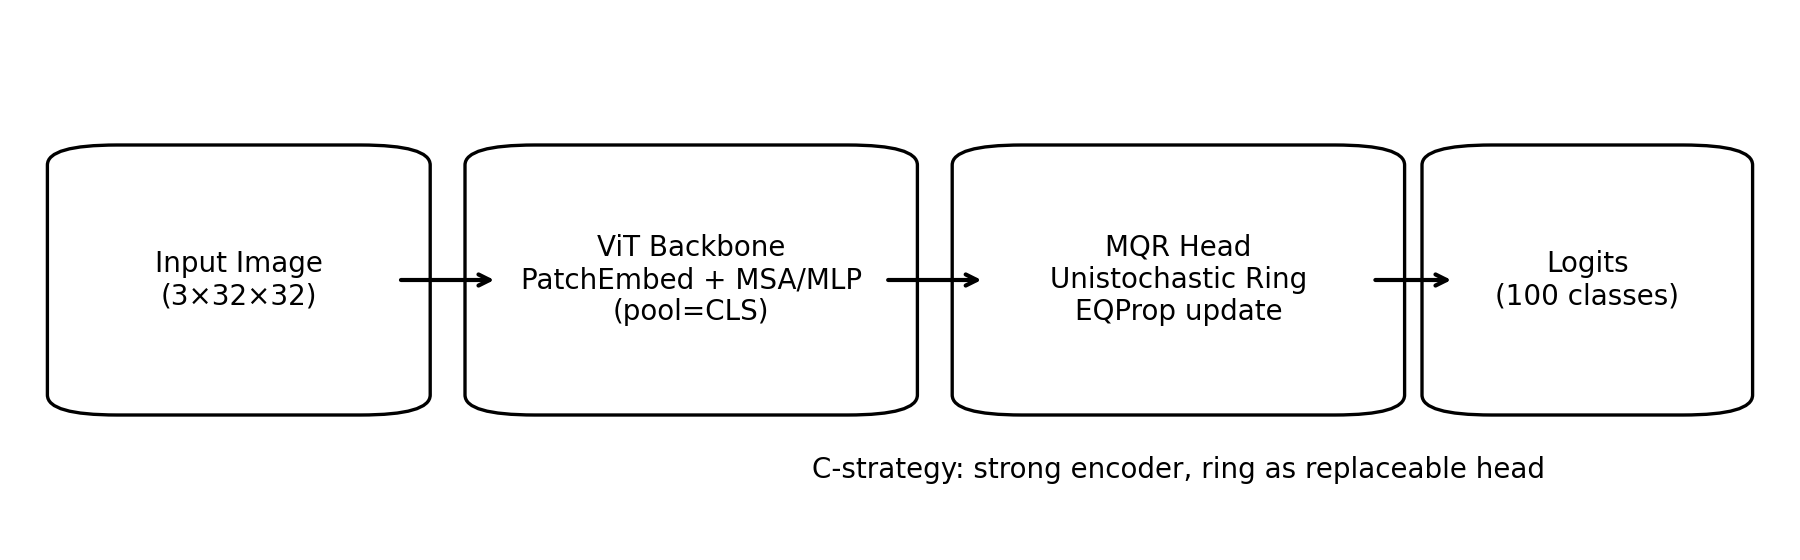
\includegraphics[width=0.98\linewidth]{figures/arch_vit_mqr.png}
\caption{C-strategy instantiation: a ViT encoder produces a feature vector, and MQR acts as a replaceable head trained by EQProp (while the encoder is trained by AdamW using gradients returned from EQProp).}
\label{fig:arch_vit_mqr}
\end{figure}

\begin{figure}[t]
\centering
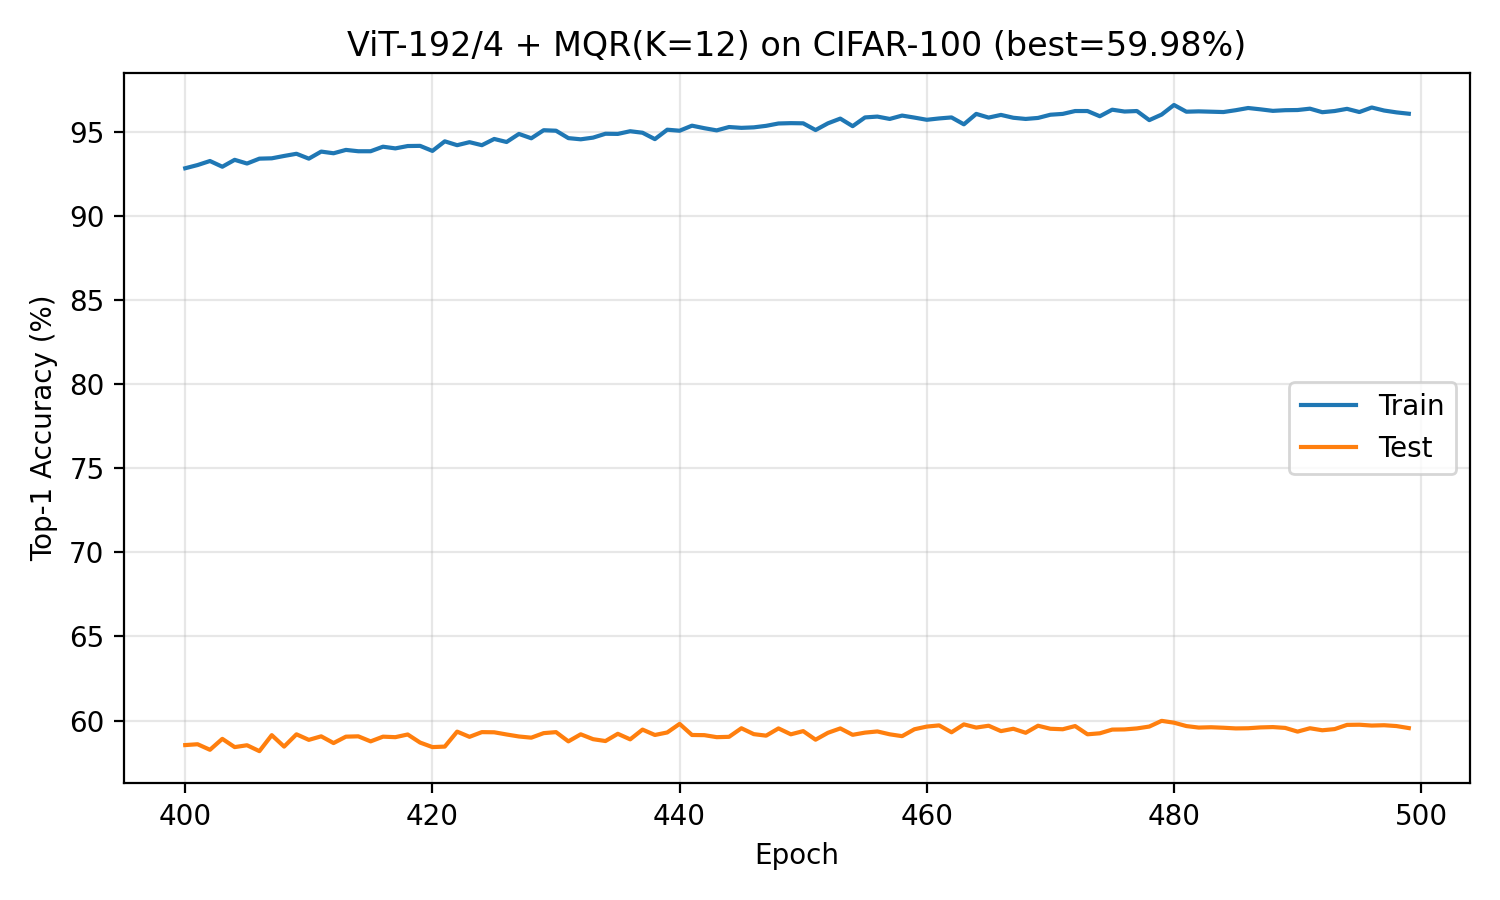
\includegraphics[width=0.98\linewidth]{figures/acc_curve_vit_mqr.png}
\caption{Accuracy curve for the best ViT-192/4 + MQR($N$=192, $K$=12) run on CIFAR-100. The model reaches \textbf{59.98\%} best test accuracy.}
\label{fig:acc_curve_vit_mqr}
\end{figure}

\begin{table}[t]
\centering
\begin{tabular}{lcc}
\toprule
\textbf{Model} & \textbf{Best Top-1 (\%)} & \textbf{Mean $\pm$ Std (\%)} \\
\midrule
ViT-192/4 + MQR head (EQProp) & 59.98 & 58.39 $\pm$ 2.10 (3 runs) \\
\bottomrule
\end{tabular}
\caption{CIFAR-100 results for the C-strategy configuration. We report the best Top-1 accuracy and the mean $\pm$ standard deviation across three repeated runs with identical hyperparameters.}
\label{tab:main_results}
\end{table}

\subsection{Controlled Ablation: Patch Encoder Pooling}
\label{sec:exp_ablation_patchpool}

To isolate the effect of spatial information flow into the ring, we run a controlled ablation with an identical patch encoder (patch size 4, embed dim 128) and identical training hyperparameters, varying only the pooling mode:
\emph{mean} pooling (ViT-style global average over patches) vs. \emph{flatten} pooling (concatenate all patch tokens).

\begin{figure}[t]
\centering
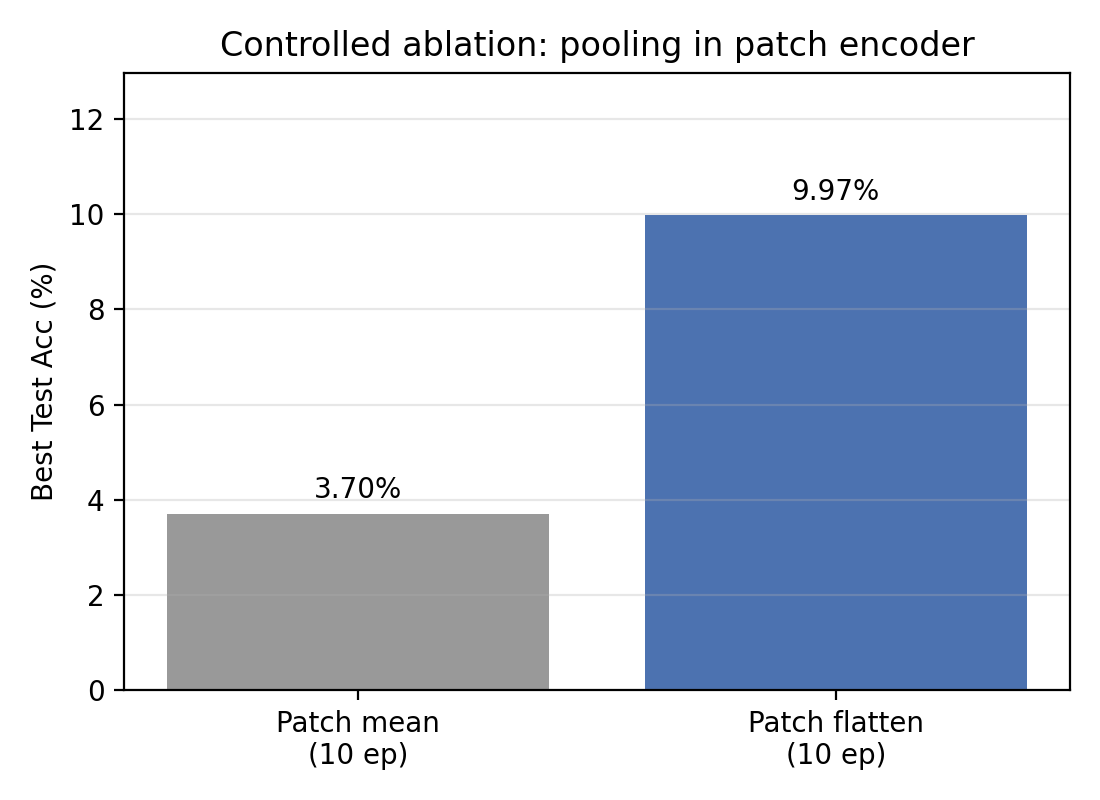
\includegraphics[width=0.72\linewidth]{figures/ablation_patch_pool_10ep.png}
\caption{Controlled ablation (10 epochs, no Mixup/CutMix): flatten pooling substantially improves early learning versus mean pooling (best test 9.97\% vs. 3.70\%). This supports the hypothesis that early MQR variants underfit when the visual front-end collapses patch structure too aggressively.}
\label{fig:ablation_patch_pool}
\end{figure}

% ========== 8. Discussion ==========
\section{Discussion}
\label{sec:discussion}

\subsection{Relationship to Quantum Computing}

While MQR uses ``quantum'' terminology, it is \textbf{not} a quantum computing algorithm. Rather, it draws inspiration from quantum mechanics:

\begin{itemize}
    \item \textbf{Unitary evolution}: In the complex unitary variant (Sec.~\ref{sec:ext_unitary}), the relaxation uses $U^\dagger$ as a norm-preserving propagator, mimicking Schrödinger dynamics. In the strict unistochastic variant, the forward coupling uses $H=|U|^2$.
    \item \textbf{Measurement}: Local projective readout (and, in Sec.~\ref{sec:ext_unitary}, magnitude measurement $|h^*|$) is analogous to quantum measurement projecting onto an observed subspace.
    \item \textbf{Phase interference}: Phase parameters are learned on the unitary manifold; in the strict unistochastic model this affects learning via $H=|U|^2$, and in the complex unitary extension phase also participates in inference through $U^\dagger$.
\end{itemize}

This quantum metaphor provides useful intuition but all computations are performed classically.

\subsection{The Möbius Metaphor}

The name ``Möbius Quantum Ring'' evokes the Möbius strip's topology---a surface with only one side. In our architecture:

\begin{itemize}
    \item The ``ring'' refers to the cyclic, non-hierarchical structure.
    \item The ``Möbius'' aspect captures the dual nature of real inference (amplitude $|U|^2$) and complex learning (phase of $U$)---two aspects of the same underlying unitary structure.
\end{itemize}

\subsection{Limitations}

\begin{itemize}
    \item \textbf{Expressivity vs. Constraint}: Unistochastic matrices form a proper subset of doubly stochastic matrices. Whether this additional structure helps or hurts expressivity is an empirical question.
    
    \item \textbf{Fixed-Point Assumption}: MQR assumes the network reaches equilibrium within $K$ steps. For complex tasks, larger $K$ may be needed.
    
    \item \textbf{Sequential Computation}: The relaxation loop is inherently sequential, though parallelizable across batch elements.
\end{itemize}

\subsection{Future Directions}

\begin{enumerate}
    \item \textbf{Continuous-Time Formulation}: Replace discrete relaxation with neural ODEs for adaptive computation.
    
    \item \textbf{Structured Unitary Matrices}: Use block-diagonal or sparse unitary matrices to reduce complexity.
    
    \item \textbf{Multi-Ring Architectures}: Stack multiple MQR modules with different time scales.
\end{enumerate}

% ========== 9. Conclusion ==========
\section{Conclusion}
\label{sec:conclusion}

We have introduced the Möbius Quantum Ring (MQR), a novel neural architecture that combines the stability guarantees of doubly stochastic matrices with the geometric elegance of unitary group parameterization. By parameterizing weights through the unistochastic manifold ($H = |U|^2$), MQR achieves:

\begin{enumerate}
    \item \textbf{Implicit Normalization}: No iterative Sinkhorn projection required.
    \item \textbf{Guaranteed Stability}: Contraction mapping ensures unique fixed-point convergence.
    \item \textbf{Efficient Learning}: Holomorphic Equilibrium Propagation enables BPTT-free training via Lie algebra updates.
\end{enumerate}

The MQR architecture offers a new paradigm for designing stable, expressive neural networks, bridging concepts from differential geometry, quantum mechanics, and deep learning.

% ========== Appendix ==========
\appendix

\section{Detailed Proofs}
\label{app:proofs}

\subsection{Proof of Proposition~\ref{prop:cayley}}

Let $A^\dagger = -A$ (skew-Hermitian). We show $(I+A)$ is invertible and $U = (I-A)(I+A)^{-1}$ is unitary.

\textbf{Invertibility:} Suppose $(I+A)v = 0$ for some $v \neq 0$. Then $v = -Av$, so:
\begin{equation}
v^\dagger v = -v^\dagger A v = -v^\dagger A v
\end{equation}
But $v^\dagger A v$ is purely imaginary (since $(v^\dagger A v)^* = v^\dagger A^\dagger v = -v^\dagger A v$). Thus $v^\dagger v = 0$, contradicting $v \neq 0$.

\textbf{Unitarity:} See proof in Section~\ref{sec:preliminaries}.

\subsection{Convergence Rate Analysis}

\begin{proposition}
Starting from $h_0 = 0$, after $t$ iterations:
\begin{equation}
\|h_t - h^*\| \leq (1-\alpha)^t \|h^*\|
\end{equation}
Thus convergence is exponential with rate $1-\alpha$.
\end{proposition}

\begin{proof}
We have $h_{t+1} - h^* = (1-\alpha)H^T(h_t - h^*)$. Iterating:
\begin{equation}
h_t - h^* = [(1-\alpha)H^T]^t (h_0 - h^*) = -[(1-\alpha)H^T]^t h^*
\end{equation}
Taking norms: $\|h_t - h^*\| \leq (1-\alpha)^t \|h^*\|$.
\end{proof}

\section{Implementation Details}
\label{app:implementation}

\subsection{Numerical Stability}

For the Cayley transform $(I-A)(I+A)^{-1}$, we use \texttt{torch.linalg.solve}:
\begin{verbatim}
U = torch.linalg.solve(I + A, I - A)
\end{verbatim}
This is numerically stable and avoids explicit matrix inversion.

\subsection{Gradient Flow}

During training with autograd, gradients flow through:
\begin{enumerate}
    \item Readout: $\nabla_{W_{readout}}\LL$
    \item Fixed point: implicit differentiation via adjoint method
    \item Cayley transform: automatic differentiation through \texttt{linalg.solve}
\end{enumerate}

The Holomorphic Equilibrium Propagation algorithm provides an alternative that avoids storing the full computation graph.

\subsection{Practical Switches in the Reference Implementation}
\label{app:impl_switches}

Our reference code (\texttt{mqr/ring.py}, \texttt{train\_mobius\_cifar100.py}) preserves the strict unistochastic MQR as the default, and exposes the following optional switches described in Sec.~\ref{sec:extensions}:
\begin{itemize}
    \item \textbf{Nonlinear injection / state activation}: \texttt{inj\_activation} (none/relu/tanh/gelu) and \texttt{state\_activation} (none/relu/tanh). For 1-Lipschitz $\sigma$, the contraction proof remains valid (Sec.~\ref{sec:ext_nonlinear}).
    \item \textbf{Patch embedding front-end}: \texttt{image\_encoder=patch} with \texttt{patch\_size} and \texttt{patch\_embed\_dim}, pooled by mean or flattened (Sec.~\ref{sec:ext_patch}).
    \item \textbf{Self-retention mixing}: \texttt{h\_mix\_beta} (and optional learning of $\beta$) implements $H_{\text{eff}}=(1-\beta)I+\beta H$ (Sec.~\ref{sec:ext_beta}).
    \item \textbf{Complex unitary inference}: \texttt{dynamics\_mode=unitary} with \texttt{measurement=abs} enables phase-participating inference (Sec.~\ref{sec:ext_unitary}).
\end{itemize}

% ========== References ==========
\bibliographystyle{plainnat}
\begin{thebibliography}{99}

\bibitem[Arjovsky et al.(2016)]{arjovsky2016unitary}
M.~Arjovsky, A.~Shah, and Y.~Bengio.
\newblock Unitary evolution recurrent neural networks.
\newblock In \emph{ICML}, 2016.

\bibitem[Ba et al.(2016)]{ba2016layer}
J.~L. Ba, J.~R. Kiros, and G.~E. Hinton.
\newblock Layer normalization.
\newblock \emph{arXiv preprint arXiv:1607.06450}, 2016.

\bibitem[Bai et al.(2019)]{bai2019deep}
S.~Bai, J.~Z. Kolter, and V.~Koltun.
\newblock Deep equilibrium models.
\newblock In \emph{NeurIPS}, 2019.

\bibitem[Bengtsson \& {\.Z}yczkowski(2005)]{bengtsson2005birkhoff}
I.~Bengtsson and K.~{\.Z}yczkowski.
\newblock On discrete structures in finite Hilbert spaces.
\newblock \emph{arXiv:quant-ph/0509194}, 2005.

\bibitem[Cho et al.(2014)]{cho2014learning}
K.~Cho, B.~Van~Merri{\"e}nboer, C.~Gulcehre, et al.
\newblock Learning phrase representations using RNN encoder-decoder for statistical machine translation.
\newblock In \emph{EMNLP}, 2014.

\bibitem[Cuturi(2013)]{cuturi2013sinkhorn}
M.~Cuturi.
\newblock Sinkhorn distances: Lightspeed computation of optimal transport.
\newblock In \emph{NeurIPS}, 2013.

\bibitem[He et al.(2016)]{he2016deep}
K.~He, X.~Zhang, S.~Ren, and J.~Sun.
\newblock Deep residual learning for image recognition.
\newblock In \emph{CVPR}, 2016.

\bibitem[Helfrich et al.(2018)]{helfrich2018orthogonal}
K.~Helfrich, D.~Willmott, and Q.~Ye.
\newblock Orthogonal recurrent neural networks with scaled Cayley transform.
\newblock In \emph{ICML}, 2018.

\bibitem[Hochreiter \& Schmidhuber(1997)]{hochreiter1997long}
S.~Hochreiter and J.~Schmidhuber.
\newblock Long short-term memory.
\newblock \emph{Neural computation}, 1997.

\bibitem[Hu et al.(2021)]{hu2021lora}
E.~J. Hu, Y.~Shen, P.~Wallis, et al.
\newblock LoRA: Low-rank adaptation of large language models.
\newblock \emph{arXiv preprint arXiv:2106.09685}, 2021.

\bibitem[Huang et al.(2017)]{huang2017densely}
G.~Huang, Z.~Liu, L.~Van Der~Maaten, and K.~Q. Weinberger.
\newblock Densely connected convolutional networks.
\newblock In \emph{CVPR}, 2017.

\bibitem[Ioffe \& Szegedy(2015)]{ioffe2015batch}
S.~Ioffe and C.~Szegedy.
\newblock Batch normalization: Accelerating deep network training by reducing internal covariate shift.
\newblock In \emph{ICML}, 2015.

\bibitem[Mhammedi et al.(2017)]{mhammedi2017efficient}
Z.~Mhammedi, A.~Hellicar, A.~Rahman, and J.~Bailey.
\newblock Efficient orthogonal parametrisation of recurrent neural networks using Householder reflections.
\newblock In \emph{ICML}, 2017.

\bibitem[Amos \& Kolter(2017)]{amos2017optnet}
B.~Amos and J.~Z. Kolter.
\newblock OptNet: Differentiable optimization as a layer in neural networks.
\newblock In \emph{ICML}, 2017.

\bibitem[Sander et al.(2022)]{sander2022sinkformers}
M.~E. Sander, P.~Ablin, M.~Blondel, and G.~Peyré.
\newblock Sinkformers: Transformers with doubly stochastic attention.
\newblock In \emph{AISTATS}, 2022.

\bibitem[Scellier \& Bengio(2017)]{scellier2017equilibrium}
B.~Scellier and Y.~Bengio.
\newblock Equilibrium propagation: Bridging the gap between energy-based models and backpropagation.
\newblock \emph{Frontiers in computational neuroscience}, 2017.

\bibitem[Sinkhorn(1967)]{sinkhorn1967concerning}
R.~Sinkhorn.
\newblock Concerning nonnegative matrices and doubly stochastic matrices.
\newblock \emph{Pacific Journal of Mathematics}, 1967.

\bibitem[Srivastava et al.(2015)]{srivastava2015highway}
R.~K. Srivastava, K.~Greff, and J.~Schmidhuber.
\newblock Highway networks.
\newblock \emph{arXiv preprint arXiv:1505.00387}, 2015.

\bibitem[Wang et al.(2025)]{wang2025sparse}
Y.~Wang et al.
\newblock Native sparse attention: Hardware-aligned and efficient sparse attention.
\newblock \emph{DeepSeek Technical Report}, 2025.

\bibitem[Wisdom et al.(2016)]{wisdom2016full}
S.~Wisdom, T.~Powers, J.~Hershey, J.~Le~Roux, and L.~Atlas.
\newblock Full-capacity unitary recurrent neural networks.
\newblock In \emph{NeurIPS}, 2016.

\end{thebibliography}

\end{document}
